%%%%%%%%%%%%%%%%%%%%%%%%%%%%%%%%%%%%%%%%%%%%%%%%%%%%%%%%%%%%%%%%%%%%%%
% LaTeX Example: Project Report
%
% Source: http://www.howtotex.com
%
% Feel free to distribute this example, but please keep the referral
% to howtotex.com
% Date: March 2011
%
%%%%%%%%%%%%%%%%%%%%%%%%%%%%%%%%%%%%%%%%%%%%%%%%%%%%%%%%%%%%%%%%%%%%%%
% How to use writeLaTeX:
%
% You edit the source code here on the left, and the preview on the
% right shows you the result within a few seconds.
%
% Bookmark this page and share the URL with your co-authors. They can
% edit at the same time!
%
% You can upload figures, bibliographies, custom classes and
% styles using the files menu.
%
% If you're new to LaTeX, the wikibook is a great place to start:
% http://en.wikibooks.org/wiki/LaTeX
%
%%%%%%%%%%%%%%%%%%%%%%%%%%%%%%%%%%%%%%%%%%%%%%%%%%%%%%%%%%%%%%%%%%%%%%
% Edit the title below to update the display in My Documents
%\title{Project Report}
%
%%% Preamble
\documentclass[paper=a4, fontsize=11pt]{scrartcl}
\usepackage[utf8x]{inputenc}

\usepackage{fourier}

\usepackage[portuguese]{babel}															% English language/hyphenation
\usepackage[protrusion=true,expansion=true]{microtype}
\usepackage{amsmath,amsfonts,amsthm} % Math packages
\usepackage[pdftex]{graphicx}
\usepackage{url}
\usepackage{multirow}
\usepackage{hyperref}
\usepackage{listings}
\usepackage{xcolor}
\usepackage{graphicx}
\usepackage{float}

%%% Custom sectioning
\usepackage{sectsty}
\allsectionsfont{\centering \normalfont\scshape}


%%% Custom headers/footers (fancyhdr package)
\usepackage{fancyhdr}
\pagestyle{fancyplain}
\fancyhead{}											% No page header
\fancyfoot[L]{}											% Empty
\fancyfoot[C]{}											% Empty
\fancyfoot[R]{\thepage}									% Pagenumbering
\renewcommand{\headrulewidth}{0pt}			% Remove header underlines
\renewcommand{\footrulewidth}{0pt}				% Remove footer underlines
\setlength{\headheight}{13.6pt}


%%% Equation and float numbering
\numberwithin{equation}{section}		% Equationnumbering: section.eq#
\numberwithin{figure}{section}			% Figurenumbering: section.fig#
\numberwithin{table}{section}				% Tablenumbering: section.tab#


\lstset{ %
	backgroundcolor=\color{white},   % choose the background color; you must add \usepackage{color} or \usepackage{xcolor}
	basicstyle=\footnotesize,        % the size of the fonts that are used for the code
	breakatwhitespace=false,         % sets if automatic breaks should only happen at whitespace
	breaklines=true,                 % sets automatic line breaking
	captionpos=b,                    % sets the caption-position to bottom
	commentstyle=\color{red},    % comment style
	extendedchars=true,              % lets you use non-ASCII characters; for 8-bits encodings only, does not work with UTF-8
	frame=single,                    % adds a frame around the code
	keepspaces=true,                 % keeps spaces in text, useful for keeping indentation of code (possibly needs columns=flexible)
	keywordstyle=\color{blue},       % keyword style
	language=C,                 % the language of the code
	otherkeywords={func, :=, ++, sync, ==},            % if you want to add more keywords to the set
	numbers=left,                    % where to put the line-numbers; possible values are (none, left, right)
	numbersep=10pt,                   % how far the line-numbers are from the code
	numberstyle=\tiny\color{gray}, % the style that is used for the line-numbers
	%rulecolor=\color{black},         % if not set, the frame-color may be changed on line-breaks within not-black text (e.g. comments (green here))
	showspaces=false,                % show spaces everywhere adding particular underscores; it overrides 'showstringspaces'
	showstringspaces=false,          % underline spaces within strings only
	showtabs=false,                  % show tabs within strings adding particular underscores
	tabsize=2,                       % sets default tabsize to 2 spaces
}

%%% Maketitle metadata
\newcommand{\horrule}[1]{\rule{\linewidth}{#1}} 	% Horizontal rule

\title{
		%\vspace{-1in}
		\usefont{OT1}{bch}{b}{n}
		\normalfont \normalsize \textsc{Instituto de Matemática e Estatística\\Universidade de São Paulo} \\ [25pt]
		\horrule{0.5pt} \\[0.4cm]
		\huge EP3 - MAC0438 \\
		\horrule{2pt} \\[0.5cm]
}
\author{
		\normalfont 								\normalsize
        João Marco Maciel da Silva 7577598\\
        \normalsize
        \today
}
\date{}


%%% Begin document
\begin{document}
\maketitle
\section{Filósofos Famintos}
	Foram feitos, não 2 quantidades diferentes, mas 3.\\
	Com 4 filósofos, 318 filósofos e 954 filósofos.\\
	No texto abaixo são apresentados apenas os casos com 4 e com 954 filósofos.
	Cada um dos 6 testes foram rodados 50 vezes. e o resultado abaixo representa a média deles.\\
	Todos os testes foram realizados em um terminal linux sem interface gráfica.\\
	O resultado integral dos testes, inclusíve o caso com 318 filósofos, pode ser encontrado \href{https://docs.google.com/spreadsheets/d/1JswsKe4sCJIXDUoLzpxeijnz9dtqEFNVYMwKC01sZhg/edit?usp=sharing}{aqui}.\\

\pagebreak
\subsection{Entrada Simples - Poucos Filósofos}
	\begin{tabular}{ll}
		Arquivo & sampleSmall\\
		Número de Filósofos& 4\\
		Pesos& 2, 8, 4, 6\\
		Refeições servidas em cada experimento& 10000\\
	\end{tabular}

\subsubsection{Modo U}
	\begin{tabular}{ll}
		Tempo médio de cada rodada& 32,41\\
		Desvio padrão do tempo de cada rodada& 0.08\\
		Desvio padrão médio do número de pratos comidos& 10,4\\
	\end{tabular}

	\begin{figure}[H]
		\centering
		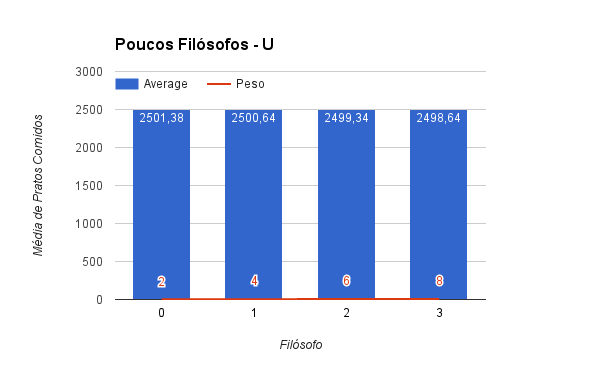
\includegraphics[width=0.9\textwidth]{image5}
		\caption{}
		\label{image5}
	\end{figure}

	No gráfico \ref{image5} percebemos que o número de pratos comidos é bem semelhante ao caso perfeito. Não é exatamente perfeito pois no modo U não há controle nenhum sobre a saciedade dos filósofos.
\pagebreak
\subsubsection{Modo P}
\begin{tabular}{ll}
	Tempo médio de cada rodada& 46,28\\
	Desvio padrão do tempo de cada rodada& 0,15\\
	Desvio padrão médio do número de pratos comidos& 0\\
\end{tabular}

\begin{figure}[H]
	\centering
	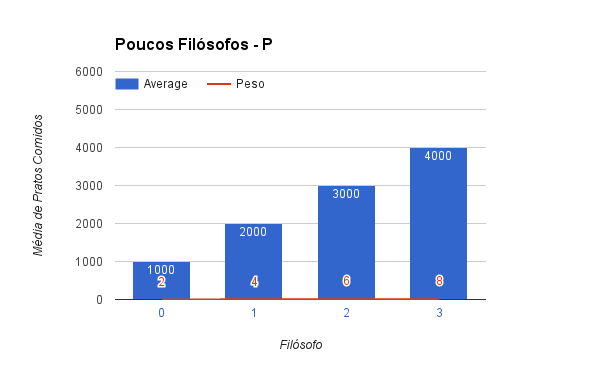
\includegraphics[width=0.9\textwidth]{image6}
	\caption{}
	\label{image6}
\end{figure}

No gráfico \ref{image6} percebemos que o número de pratos comidos é exato, pois 10000 é múltiplo do peso total, e o controle de pratos comidos é baseado na soma dos pesos.

\pagebreak
\subsection{Entrada Complexa - Muitos Filósofos}
\begin{tabular}{ll}
	Arquivo & sampleBig2\\
	Número de Filósofos& 954\\
	Pesos& 3 PAs de razão 1 de 1 a 318
	\\
	Refeições servidas em cada experimento& 1000000\\
\end{tabular}
\subsubsection{Modo U}
\begin{tabular}{ll}
	Tempo médio de cada rodada& 32,49\\
	Desvio padrão do tempo de cada rodada& 0,47\\
	Desvio padrão médio do número de pratos comidos& 7,2\\
\end{tabular}

\begin{figure}[H]
	\centering
	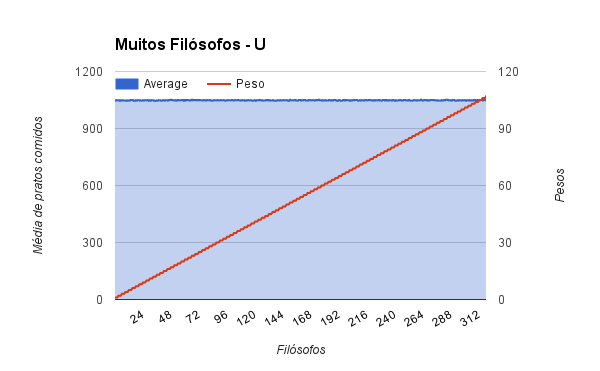
\includegraphics[width=0.9\textwidth]{image7}
	\caption{}
	\label{image7}
\end{figure}

No gráfico \ref{image7} percebemos que o número de pratos comidos é bem semelhante ao caso perfeito. Não é exatamente perfeito pois no modo U não há controle nenhum sobre a saciedade dos filósofos.

\pagebreak
\subsubsection{Modo P}
\begin{tabular}{ll}
	Tempo médio de cada rodada& 41,98\\
	Desvio padrão do tempo de cada rodada& 0,81\\
	Desvio padrão médio do número de pratos comidos& 1,4\\
\end{tabular}

\begin{figure}[H]
	\centering
	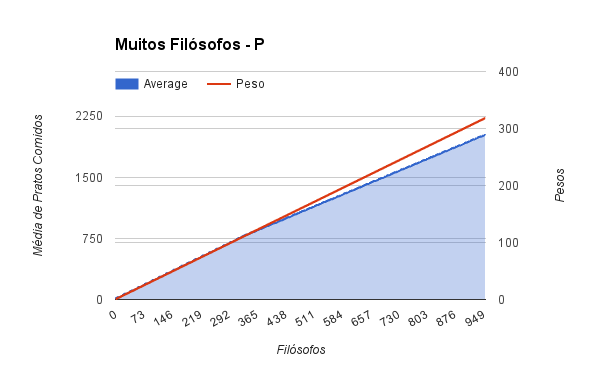
\includegraphics[width=0.9\textwidth]{image8}
	\caption{}
	\label{image8}
\end{figure}

No gráfico \ref{image8} percebemos que o número de pratos comidos parece uma linha perfeita. A diferença no final são apenas os pratos da última rodada incompleta.

\pagebreak
\section{Extras}
\subsection{Configuração da Máquina}
	Informações extraídas por \textit{dmidecode}, \textit{uname} e \textit{lsb\_release}.\\

	\begin{tabular}{lll}
		\multirow{3}{*}{Baseboard} & Type& Laptop\\
		& Manufacturer& SAMSUNG ELECTRONICS CO., LTD.\\
		& Product Name& R480/R431/R481\\
		\hline
		\multirow{6}{*}{Processor}& Family& Core i3\\
		& Max Speed& 3200MHz\\
		& Core Count& 2\\
		& Thread Count& 4\\
		& Characteristics& 64-bit capable\\
		& CPU Governor& performance\\
		\hline
		\multirow{5}{*}{Memory}& Type& DDR3\\
		& Data Width& 64 bits\\
		& Speed& 667MHz\\
		& Number of Devices& 2\\
		& Size& 2048MB x2\\
		\hline
		\multirow{3}{*}{Cache Size}& L1& 32 kB\\
		& L2& 256 kB\\
		& L3& 3072 kB\\
		\hline
		\multirow{3}{*}{uname}& OS& Linux\\
		& Kernel Release& 3.19.5-100.fc20.x86\_64\\
		& Processor type& x86\_64\\
		\hline
		\multirow{1}{*}{lsb\_release}& Description& Fedora 20\\
	\end{tabular}

Os testes foram todos feitos em um terminal sem interface gráfica

\pagebreak
\subsection{Entrada Complexa - Muitos Filósofos 2}
\begin{tabular}{ll}
	Arquivo & sampleBig\\
	Número de Filósofos& 318\\
	Pesos& PA de razão 1 de 1 a 318
	\\
	Refeições servidas em cada experimento& 1000000\\
\end{tabular}
\subsubsection{Modo U}
\begin{tabular}{ll}
	Tempo médio de cada rodada& 49,43\\
	Desvio padrão do tempo de cada rodada& 0,58\\
	Desvio padrão médio do número de pratos comidos& 13,0\\
\end{tabular}

\begin{figure}[H]
	\centering
	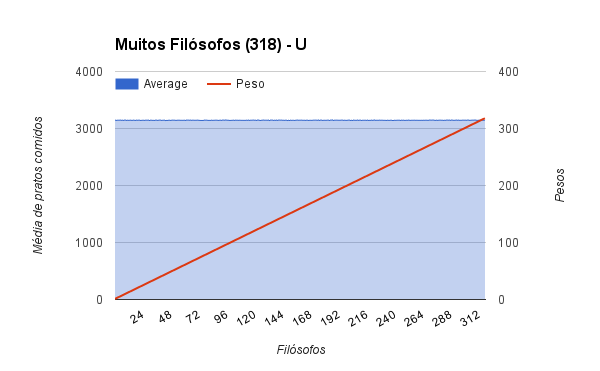
\includegraphics[width=0.9\textwidth]{image9}
	\caption{}
	\label{image9}
\end{figure}

No gráfico \ref{image9} percebemos que o número de pratos comidos é bem semelhante ao caso perfeito. Não é exatamente perfeito pois no modo U não há controle nenhum sobre a saciedade dos filósofos.

\pagebreak
\subsubsection{Modo P}
\begin{tabular}{ll}
	Tempo médio de cada rodada& 87,41\\
	Desvio padrão do tempo de cada rodada& 0,77\\
	Desvio padrão médio do número de pratos comidos& 1,5\\
\end{tabular}

\begin{figure}[H]
	\centering
	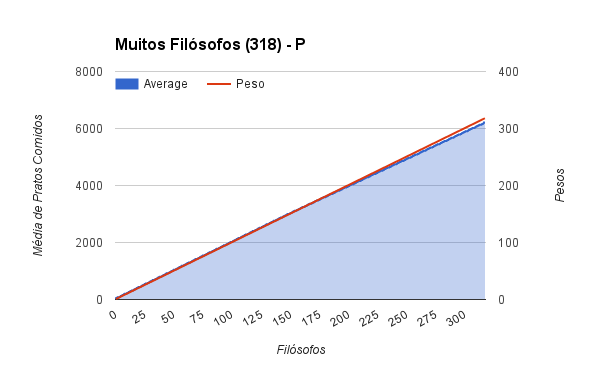
\includegraphics[width=0.9\textwidth]{image10}
	\caption{}
	\label{image10}
\end{figure}

No gráfico \ref{image10} percebemos que o número de pratos comidos parece uma linha perfeita. A diferença no final são apenas os pratos da última rodada incompleta.

\pagebreak
\subsection{Comprativo do tempo de execução}
É interessante mostrar o comparativo entre os tempo de execução.

\subsubsection{UxP}
Em todos os 3 casos percebe-se que U é mais rápido que P. Isso se deve ao fato que, por causa do controle de turnos, P passa um tempo com mais filósofos pensando quando poderiam estar consumindo o recurso(comida).

\subsubsection{4 x 318 x 954 Filósofos}
É de se esperar que até uma certa quantidade de filósofos o tempo diminua e depois aumente até valores maiores que o caso com poucos filósofos.\\
Nestes 3 testes percebe-se justamente o contrário, que o tempo aumenta e depois diminui, sendo t(954)<t(4)<t(318).\\
O resultado foi inesperado e não consegui pensar em nada que justificasse o resultado obitido.

\subsection{Geração dos gráficos}
Os gráficos e cálculos estatísticos foram feitos com ajuda do Google Spreadsheets e os dados originais podem ser encontrados \href{https://docs.google.com/spreadsheets/d/1JswsKe4sCJIXDUoLzpxeijnz9dtqEFNVYMwKC01sZhg/edit?usp=sharing}{aqui}.\\
%%% End document
\end{document}